\documentclass[cnatzke_thesis_proposal.tex]{subfiles}
\begin{document}

\chapter{Data Analysis}

%------------------------------------------
\subsection{First Data Collection November 2017}
%------------------------------------------
Attempting to observe two-photon decay with GRIFFIN is very challenging technically and requires multiple iterations with each subsequent data collection reducing relevant backgrounds. 
The first attempt at measuring two-photon decay with GRIFFIN occurred in November 2017 using a $^{90}$Sr source already present at TRIUMF and was used to evaluate the feasibility of measuring two-photon transitions and assess the background level in the array. 
All sixteen GRIFFIN clovers were present in the array in high-efficiency mode, the BGO suppression shields had not been installed yet, and the $^{90}$Sr puck source was roughly aligned to the centre of the array using a source holder. 
X-ray absorbers, composed of 0.1 mm layer of Tantalum (Ta), 0.25 mm layer of Tin (Sn), and 0.25 mm layer of Copper (Cu), were placed in front of the clover faces with the Cu layer facing the clover. 
DAQ rates are detailed in \ref{tab:daq_rates}.

\begin{table}[]
  \centering
  \begin{tabular}{ccccc}
                    & Source          & Crystal Rate & Total Array Rate & Data Rate \\ \hline
  \textbf{Nov 2017} & $^{90}$Sr       & 15-22 kHz    & 625 kHz          & 26.6 MB/s \\ \hline
  \textbf{Oct 2018} & $^{90}$Sr       & 4-8 kHz      & 305 kHz          & 12.9 MB/s \\ \hline
  \textbf{Dec 2019} & $^{90}$Sr       & 2-2.5 kHz    & 20 kHz           & 1.0 MB/s  \\ 
                    & Room Background & 200 Hz       & -                & 0.2 MB/s  \\ \hline
  \end{tabular}
  \caption{DAQ data rates for the three data collections}
  \label{tab:daq_rates}
\end{table}


%------------------------------------------
\subsection{Data Collection October 2019}
%------------------------------------------
% new custom souce holder. 
%------------------------------------------
\subsubsection{Custom Source Holder}
%------------------------------------------

Prior to this data collection the $^{90}$Sr source had the activity mounted on an industrial ceramic backing causing a significant low-energy background that obscured any two-photon peak. 
The high beta activity of the source caused the Tungsten dopant in the ceramic to flouresce x-rays, of characteristic energy 57 and 65 keV, measured primarily in detectors directly behind the ceramic backing of the source. 
Furthermore, the ceramic and the bronze source holder were made of sufficiently high-Z materials such that the Bremsstrahlung radiation from the interaction of the betas released from the source masked any two-photon signal that GRIFFIN could measure. 

To remove the Tungsten x-rays and reduce the Bremsstrahlung radiation a new custom source was fabricated where the $^{90}$Sr activity was placed in the centre of a DELRIN (polyoxymethylene) sphere. 
A commercially obtained 20 MBq liquid Strontium Chloride, dissolved in 0.1M HCL, source was purchased and the source was evaporated into the centre of a DELRIN sphere, which was then sealed. 
Figure~\ref{fig:source_holder} shows the source holder pre-source evaporation. 
Since there is no high-Z material in the source holder the Bremsstrahlung radiation is strongly reduced compared to the original source. 

% TODO Add picture

\begin{figure}[htbp]
  \centering
  \subfloat{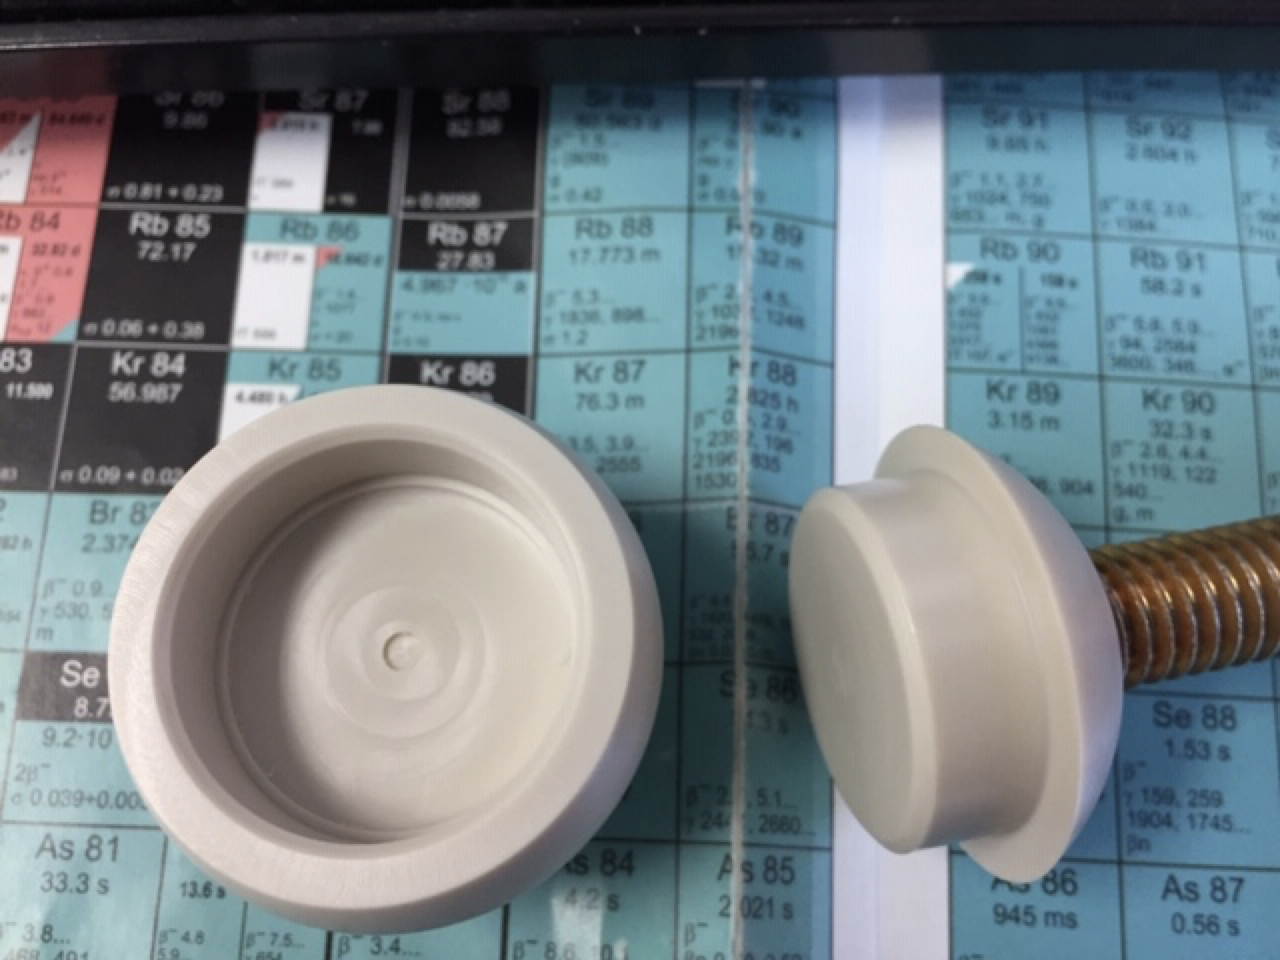
\includegraphics[height=6cm]{source_holder_open.png}}
  \qquad
  \subfloat{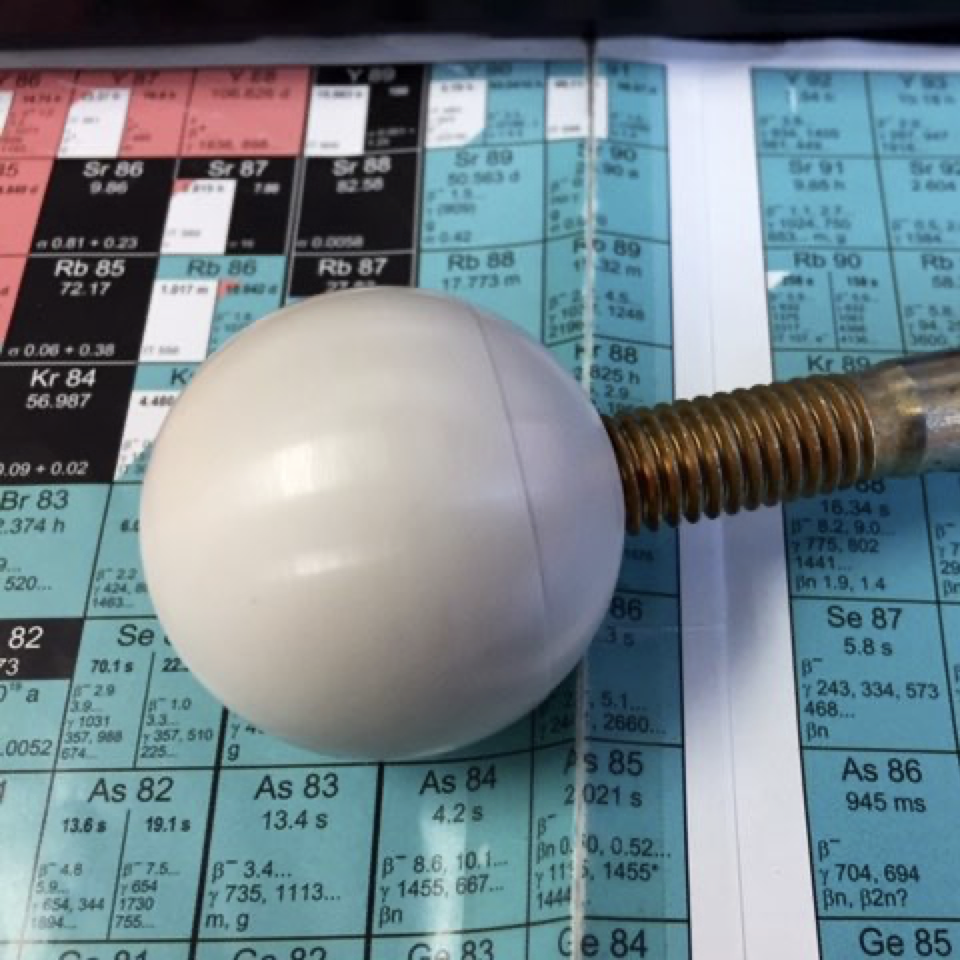
\includegraphics[height=6cm]{source_holder_closed.png}}
  \caption{
    \textit{Left:} DELRIN source holder before $^{90}$Sr activity deposit. The activity will be deposited in the centre of the larger section via evaporation of a Strontium Chloride solution. 
    \textit{Right:} DELRIN source holder with both halves closed together.
  }
  \label{fig:source_holder}
\end{figure}

A PEEK (polyetheretherketone) source holder was fabricated to hold the sphere containing the $^{90}$Sr activity in the centre of the array and the Ta/Sn/Cu X-ray absorbers were placed in the open faces of the GRIFFIN rhombicuboctahedron to increase the passive shielding of the array. This configuration is shown in the left panel of Figure~\ref{fig:source_holder_in_griffin}. The source holder was aligned using a laser point placed on the upstream beamline, shown in the right panel of Figure~\ref{fig:source_holder_in_griffin}.

\begin{figure}[htbp]
  \centering
  \subfloat{\includegraphics[height=5cm]{custom_90Sr_source.jpg}}
  \qquad
  \subfloat{\includegraphics[height=5cm]{beamline_xray_absorbers.png}}
  \caption{
    \textit{Left:} Photograph of $^{90}$Sr source and source holder aligned to the centre of GRIFFIN. Ta/Sn/Cu X-ray absorbers were placed in the opening faces of the GRIFFIN rhombicuboctahedron to help reduce room background and increase passive shielding.
    \textit{Right:} Photograph of $^{90}$Sr holder looking upstream. The red arrow points to the laser pointer used to align the source sphere.
  }
  \label{fig:source_holder_in_griffin}
\end{figure}

% todo: add comparision plot of cyclotron on vs off?
Unlike the previous data collections this dataset was taking during the TRIUMF annual shutdown, when TRIUMF shuts down the main cyclotron and RIB production for maintenance and development, to reduce the neutron flux through the experimental hall. Data collection started in late December 2020 and continued through January 2021 for a total of 500 hours of source data and 300 hours of room background. The HPGe crystals were counting at 2-2.5 kHz during the source collection and 200 Hz during the room background collection, with a DAQ rate of 1 MB/s and 0.2 MB/s respectively.

\begin{table}[]
  \begin{tabular}{ccc}
                  & \textbf{Crystal Rate} & \textbf{Data Rate} \\ \hline
  $^{90}$Sr       & 2.0 - 2.5 kHz         & 1.0 MB/s           \\
  Room Background & 200 Hz                & 0.2 MB/s          
  \end{tabular}
  \caption{Crystal and DAQ rates during the December 2020 data collection}
  \label{tab:dec2020_rates}
\end{table}

The new custom source holder allowed for greater peak fidelity and completely removed the tungsten fluorescent x-rays. 
\ref{fig:dec2020_gamma_singles} is the gamma singles, using HPGe crystal energies rather than addback, energy spectrum from 506 hours of data collection.

\begin{figure}[htbp]
  \centering
  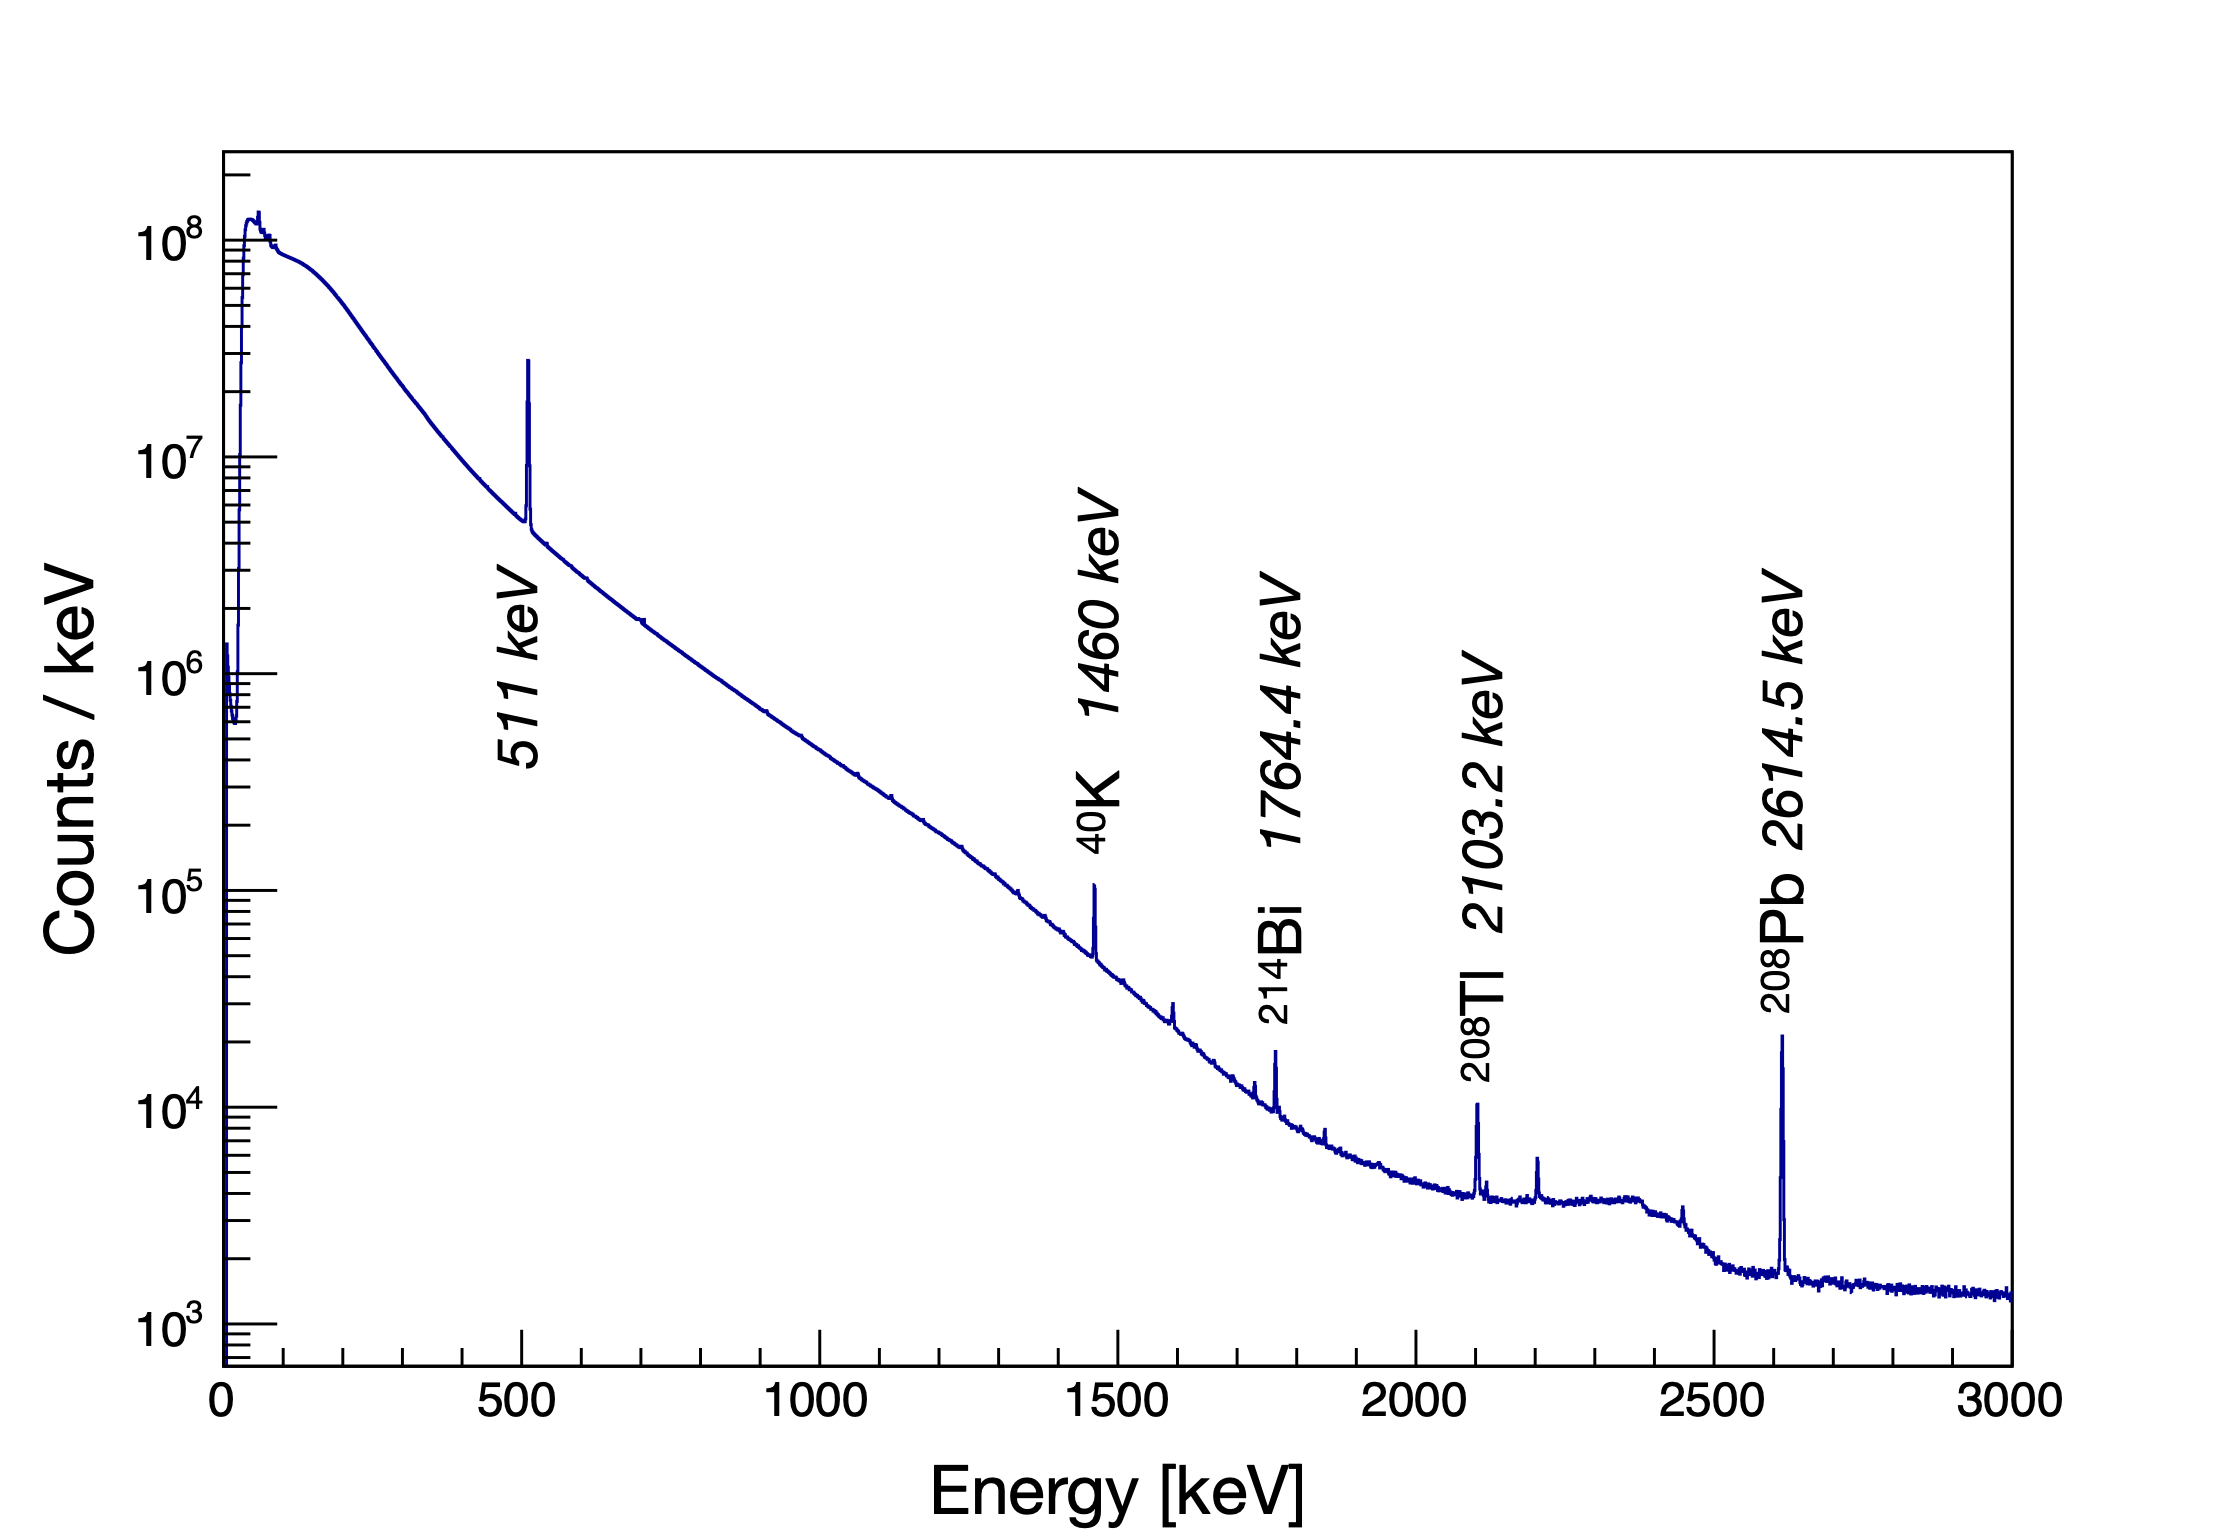
\includegraphics[width=0.95\textwidth]{dec2020_gamma_singles.png}
  \caption{$\gamma$-ray singles energy spectrum from 506 hours of $^{90}$Sr source data collection. Prominent room background peaks have been labeled.}
  \label{fig:dec2020_gamma_singles}
\end{figure}

%------------------------------------------
\subsubsection{Searching for a Two-Photon Peak}
%------------------------------------------

The two photons released during a two-photon decay event sum to the total energy of the transition, meaning the full energy of the transition should show up as a peak in a sum spectrum. 
A sum spectrum is generated by summing the energies of two incident photons together and recording their resultant sum in a histogram.
This is similar to the GRIFFIN addback algorithm, where the energy of all events detected within a single clover are summed together, but does not restrict the sum to singles events within the same clover; but rather, sums events together that were registered in different crystals regardless of if they were in the same clover of not. 
To decrease the influence of random, spurious sum peaks and provide the best chance of observing a two-photon peak only events of multiplicity two, where only two hits were recorded in the event, were used to generate the sum spectrum shown in \ref{fig:sum_spectrum_dec2019}.

\begin{figure}[htbp]
  \centering
  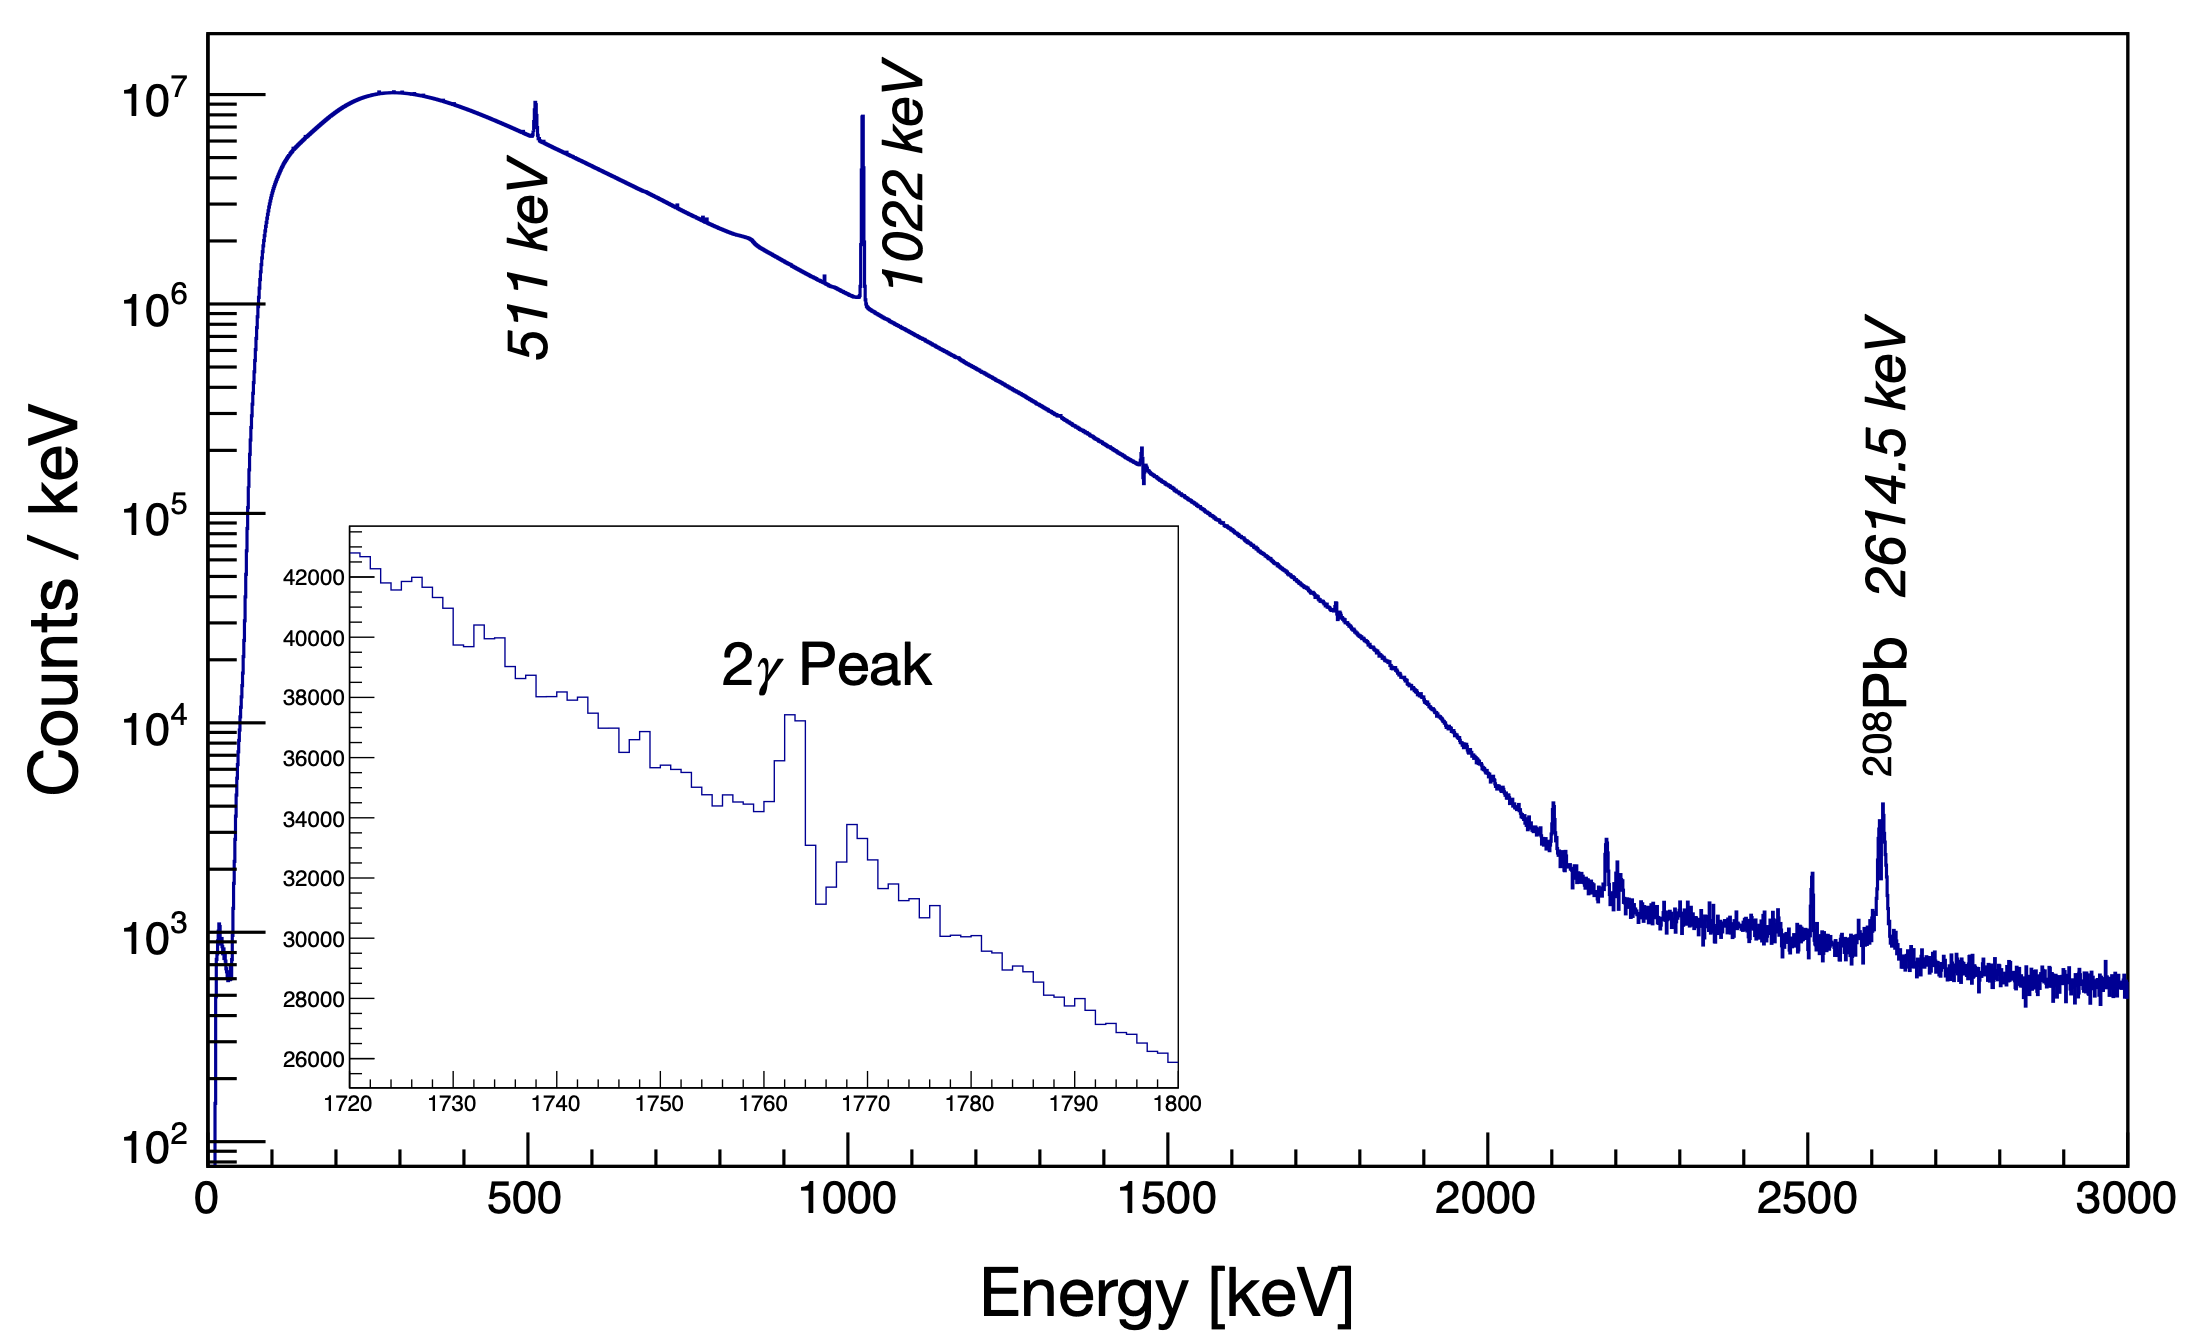
\includegraphics[width=0.95\textwidth]{sum_spectrum_dec2019.png}
  \caption{Room background subtracted $\gamma$-ray energy sum spectrum from 506 hours of $^{90}$Sr source and 300 hours of room background data. Major peaks are labeled and only events of multiplicity two were used to fill the histogram. \textit{Insert:} Focus on the region where the 1760 keV two-photon peak is expected. Here the statistical background subtraction of the 1764 keV peak from $^{214}$Bi decay can be seen.}
  \label{fig:sum_spectrum_dec2019}
\end{figure}




% ------------------------------------
\end{document}
